\section{Results}

In this section we show how long it takes to resolve a fault over the network and we compare \projname{} to \verb,malloc, in several tests.

\subsection{Fault duration}


\subsection{Malloc vs. \projname{}}

The program used to test was a matrix multiplcation program from Stanford.

\subsubsection{Fixed matrix size, varying number of threads}

In this test we kept the matrix size fixed at 200x200 and we varied the number of worker threads betweem 1 and 4.

\begin{figure}[!h]
\centering
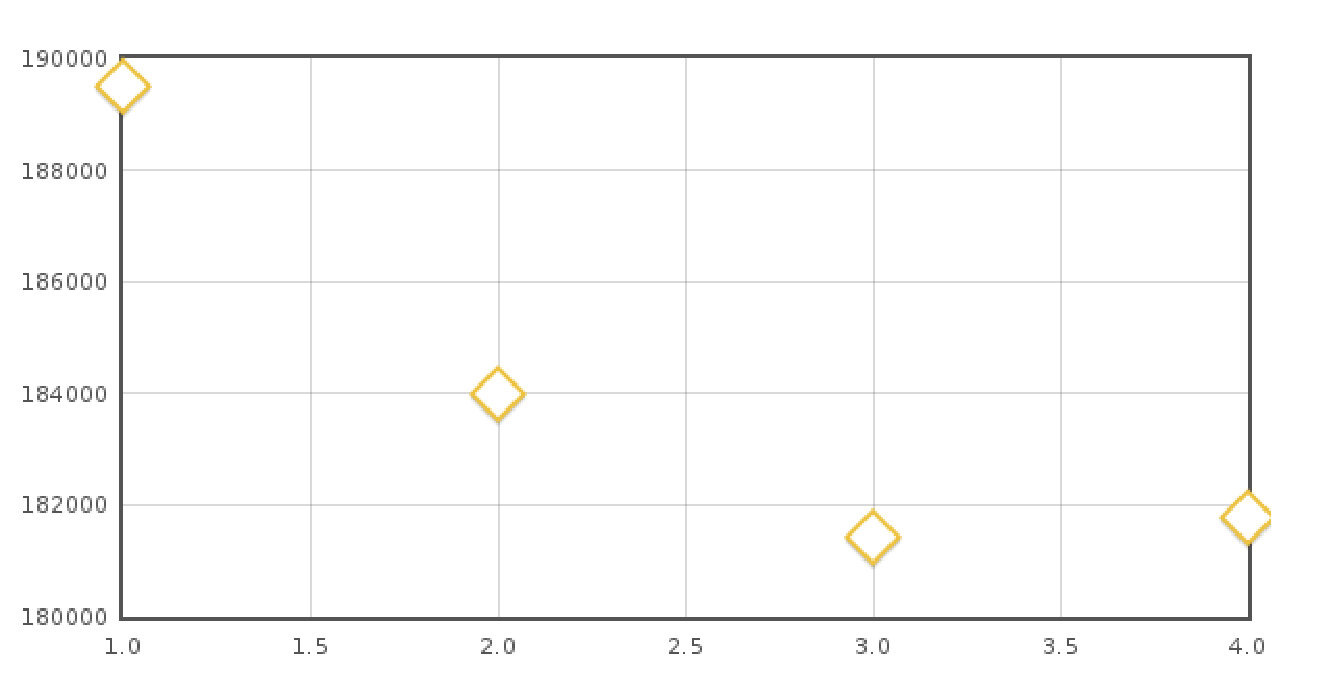
\includegraphics[scale=0.40]{images/malloc-fixed-matrix.eps}
\caption{Malloc: The x axis the number of threads used. The y axis is time to run the test in microseconds.}
\end{figure}

\begin{figure}[!h]
\centering
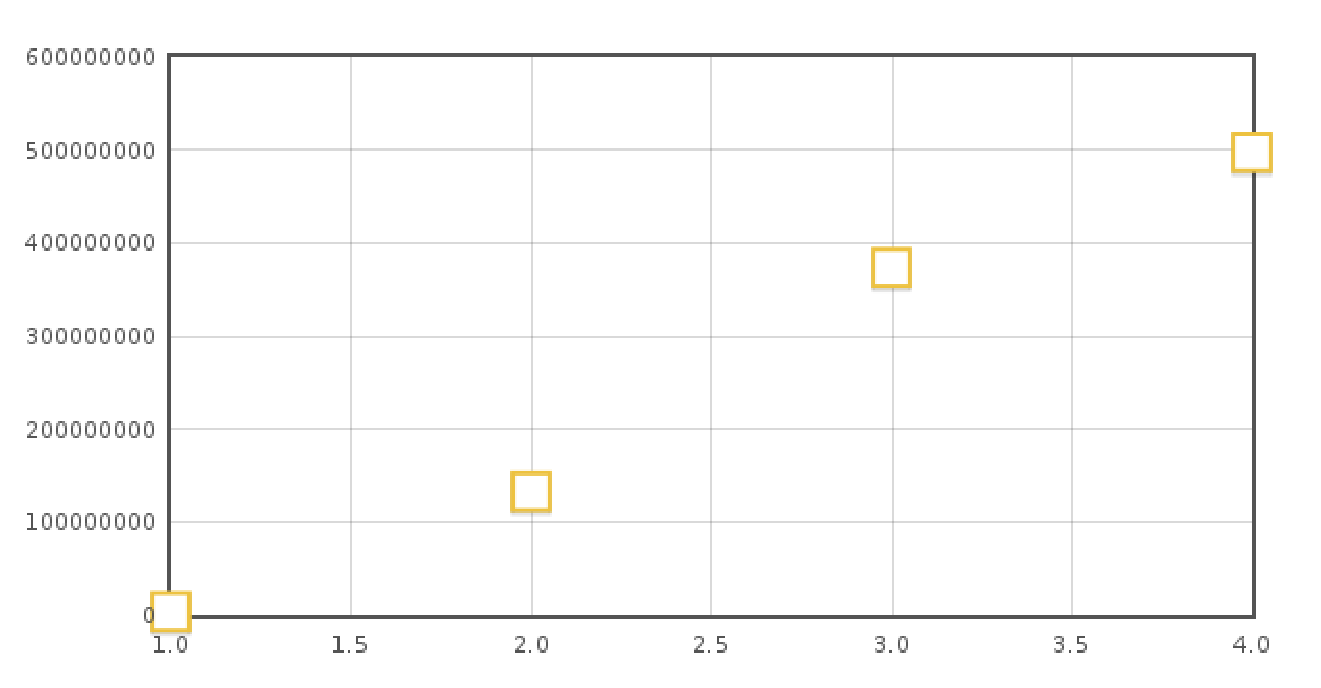
\includegraphics[scale=0.40]{images/mmult-lh-fixed-size.eps}
\caption{\projname{} with processor consistency: The x axis the number of threads used. The y axis is time to run the test in microseconds.}
\end{figure}

\begin{figure}[!h]
\centering
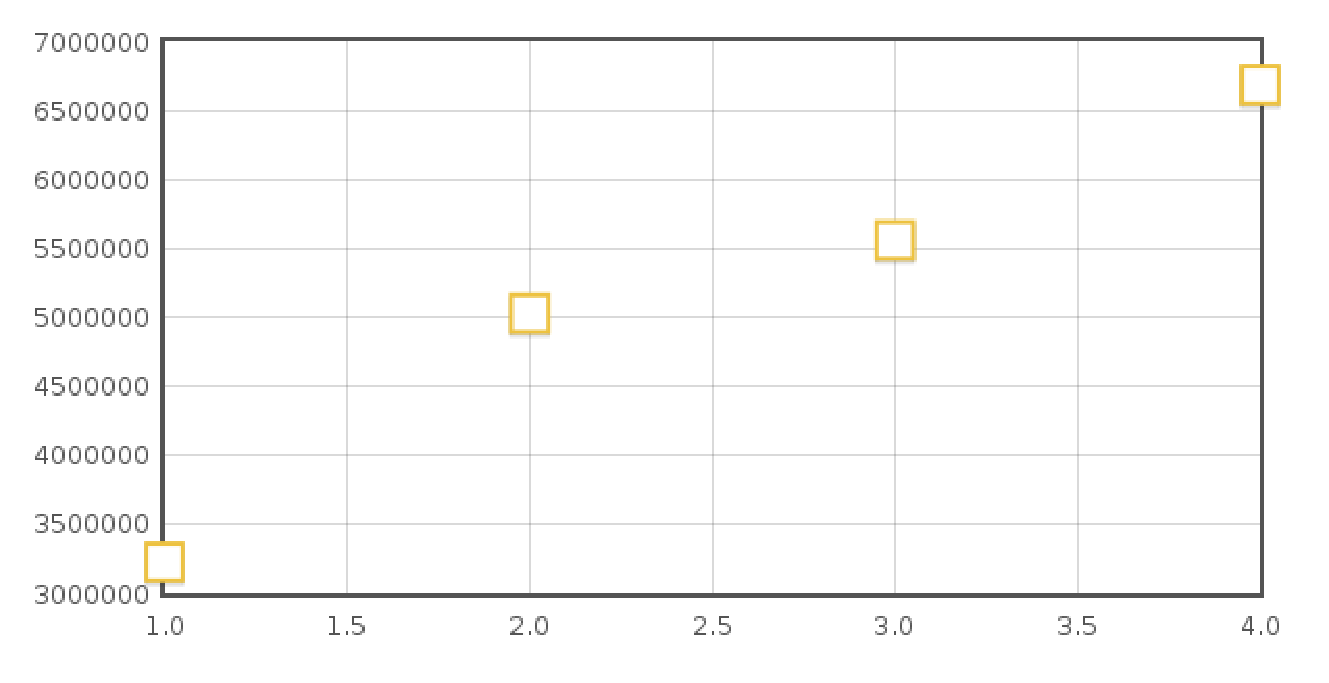
\includegraphics[scale=0.40]{images/mmlh-fixed-size.eps}
\caption{\projname{} with release consistency: The x axis is matrix size. For example, 100 refers to multiplying 2 100x100 matrixes. The y axis is time to run the test in microseconds.}
\end{figure}

\verb,Malloc, vastly outperforms \projname{} with processor consistency no matter how many threads are used.  This has to do with not having read-only pages.  Every time a worker needs to do work it invalidates all other workers copies of that page.  This ends up with the workers thrashing over pages.  It was expected when we began this test that \projname{} with processor consistency would yield worse results as the number of threads increased because of the trashing issues.

With release consistency, \projname{} achieves much better performance than processor consistency.  For 4 threads, release consistency only takes around 66 seconds.  Compared to processor consistency taking around 500 seconds.  Release consistency still loses to the \verb,malloc, version.  One reason why is because the workers end up thrashing over the write pages.

\subsubsection{Fixed thread count, varying matrix size}

In this test we kept the number of worker threads fixed at 4 and we varied the matrix size.

\begin{figure}[!h]
\centering
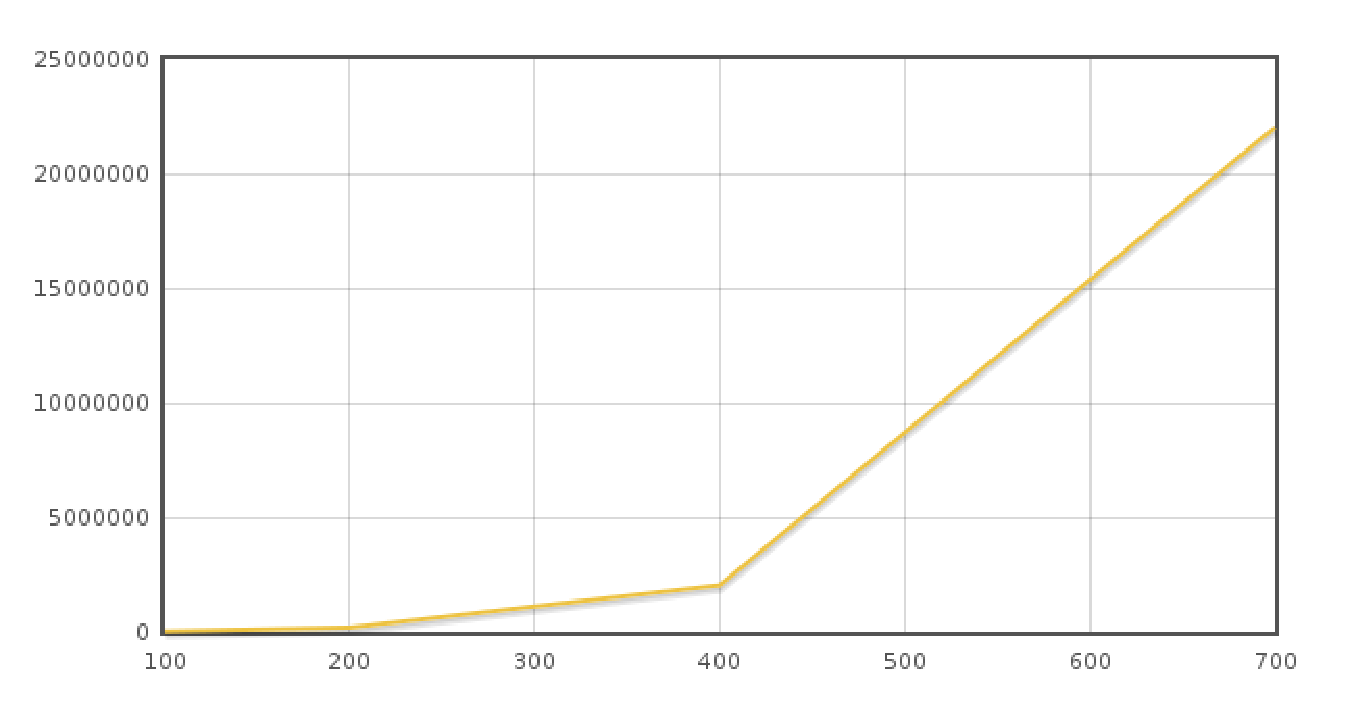
\includegraphics[scale=0.40]{images/malloc-fixed-thread.eps}
\caption{Malloc: The x axis is matrix size. For example, 100 refers to multiplying 2 100x100 matrixes. The y axis is time to run the test in microseconds.}
\end{figure}

\begin{figure}[!h]
\centering
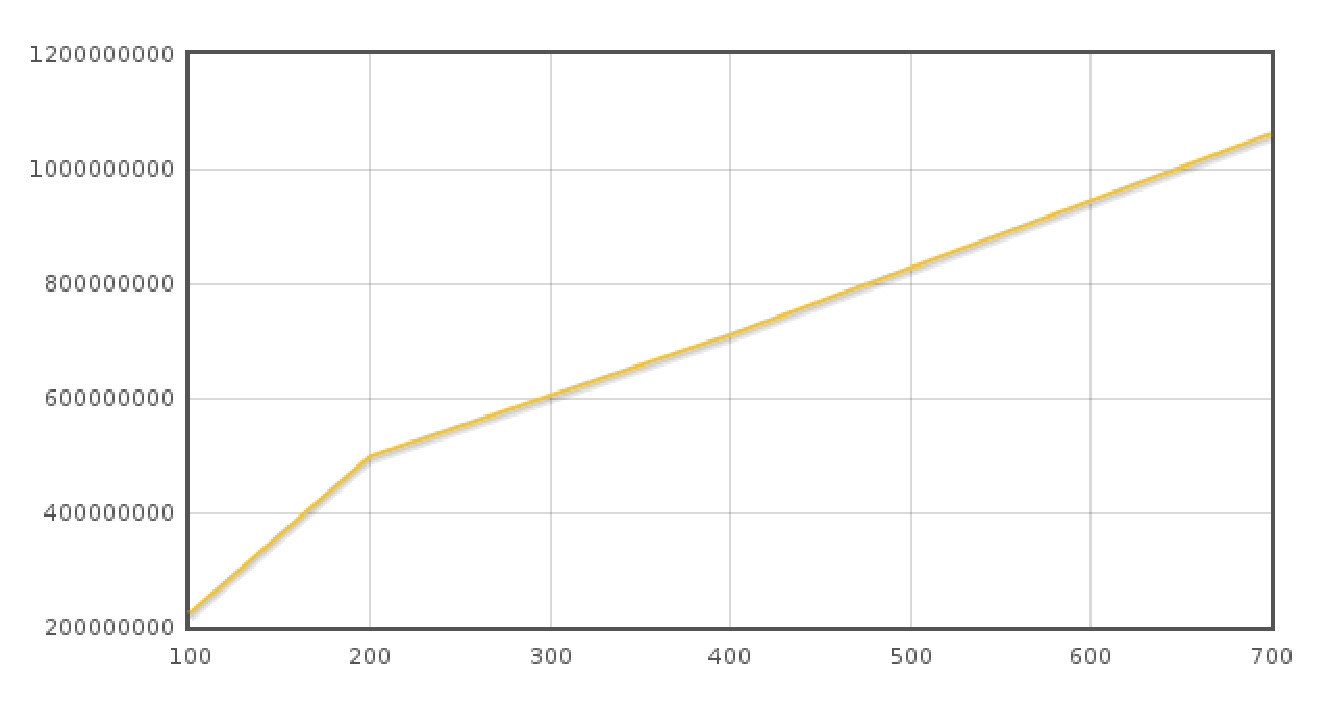
\includegraphics[scale=0.40]{images/mmult-lh-fixed-thread.eps}
\caption{\projname{} with processor consistency: The x axis is matrix size. For example, 100 refers to multiplying 2 100x100 matrixes. The y axis is time to run the test in microseconds.}
\end{figure}

\begin{figure}[!h]
\centering
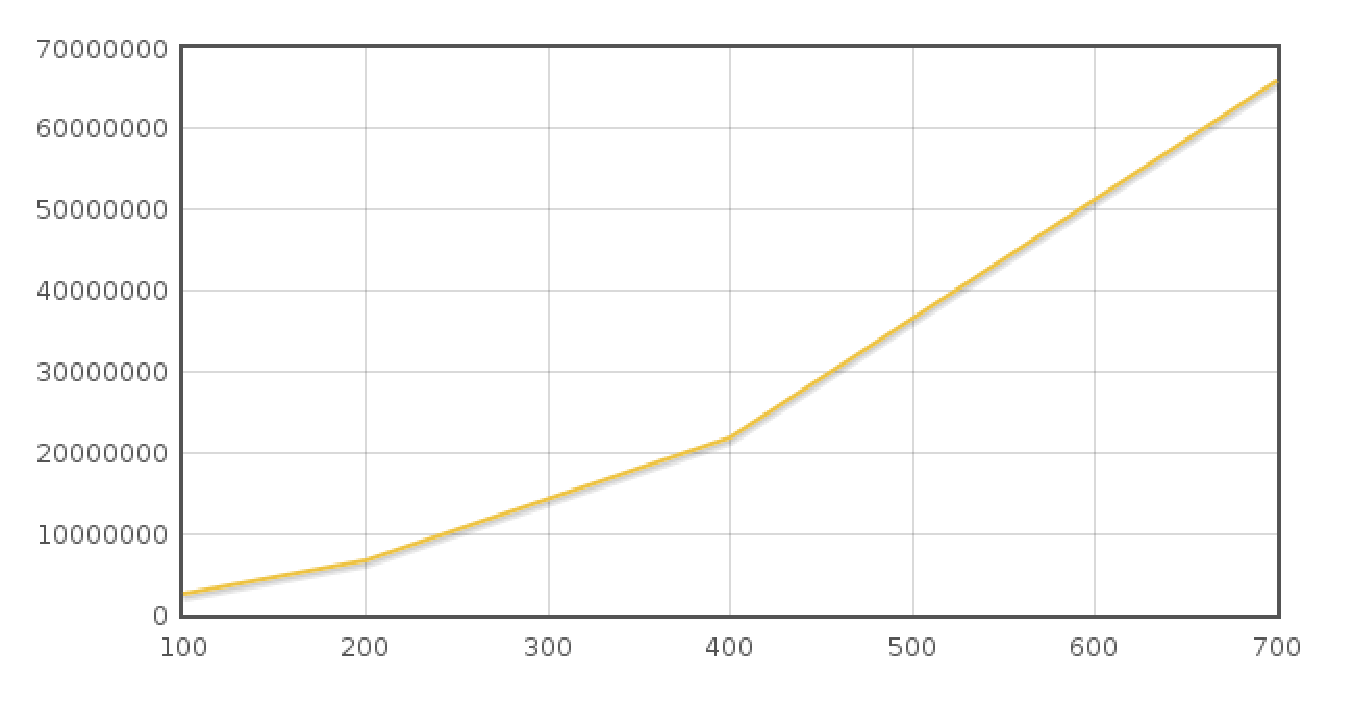
\includegraphics[scale=0.40]{images/mmlh-fixed-threads.eps}
\caption{\projname{} with release consistency: The x axis is matrix size. For example, 100 refers to multiplying 2 100x100 matrixes. The y axis is time to run the test in microseconds.}
\end{figure}

Again, like in the previous test \verb,malloc, vastly outperforms \projname{} with processor consistency at any matrix size. \projname{} with processor consistency gets hit hard by not having read only pages. It ends up transferring the 2 matrixes being multiplied a ton thereby having a horrific runtime.

With release consistency, \projname{} achieves much better performance than processor consistency. Again, release consistency still loses to the \verb,malloc, version because the workers end up thrashing over the write pages. It is still impressive that the release consistency version multiplying a 700x700 matrix finishes in around 66 seconds. The processor consistency version of the project was destroyed by that test and ended up taking over 1000 seconds.
